\chapter{Hyperspectral}

%TODO translate 
Une image hyperspectrale de la Terre acquises depuis
un porteur aérien ou spatial contient une collection de pixels
spectraux ou, de manière équivalente, une collection de bandes
spectrales.

\begin{figure}[h]
  \centering
  \includegraphics[width=0.7\textwidth]{Cube_HPX.eps}
  \itkcaption[Hyperspectral cube]{Illustration d'un cube hyperspectral, d'un pixel spectral et
d'une bande spectrale.}
  \label{fig:cube}
\end{figure}

Le cube hyperspectral \ref{fig:cube} acquis est une image de
radiance, chaque pixel spectral contient une information spectrale
fine qui dépend : 

\begin{enumerate}
\item{Du spectre de la source lumineuse (en pratique, le
soleil) et des perturbations atmosphériques.}
\item{Des réponses spectrales
des différents matériaux présents dans la zone de recouvrement et de la nature de leur mélange.}
\end{enumerate}

Des traitements préliminaires de
correction atmosphérique permettent d'estimer un cube de réflectance
spectrale par soustraction de l'information extrinsèque à la
scène. 

\section{Unmixing}

L'information de réflectance ne dépend que des spectres de
réflectance des matériaux de la scène. Lorsque le mélange entre les
matériaux est macroscopique, le modèle de mélange linéaire de spectres
est généralement admis. La scène imagée a typiquement l'allure
illustrée ci-après :

\begin{figure}[h]
  \centering
  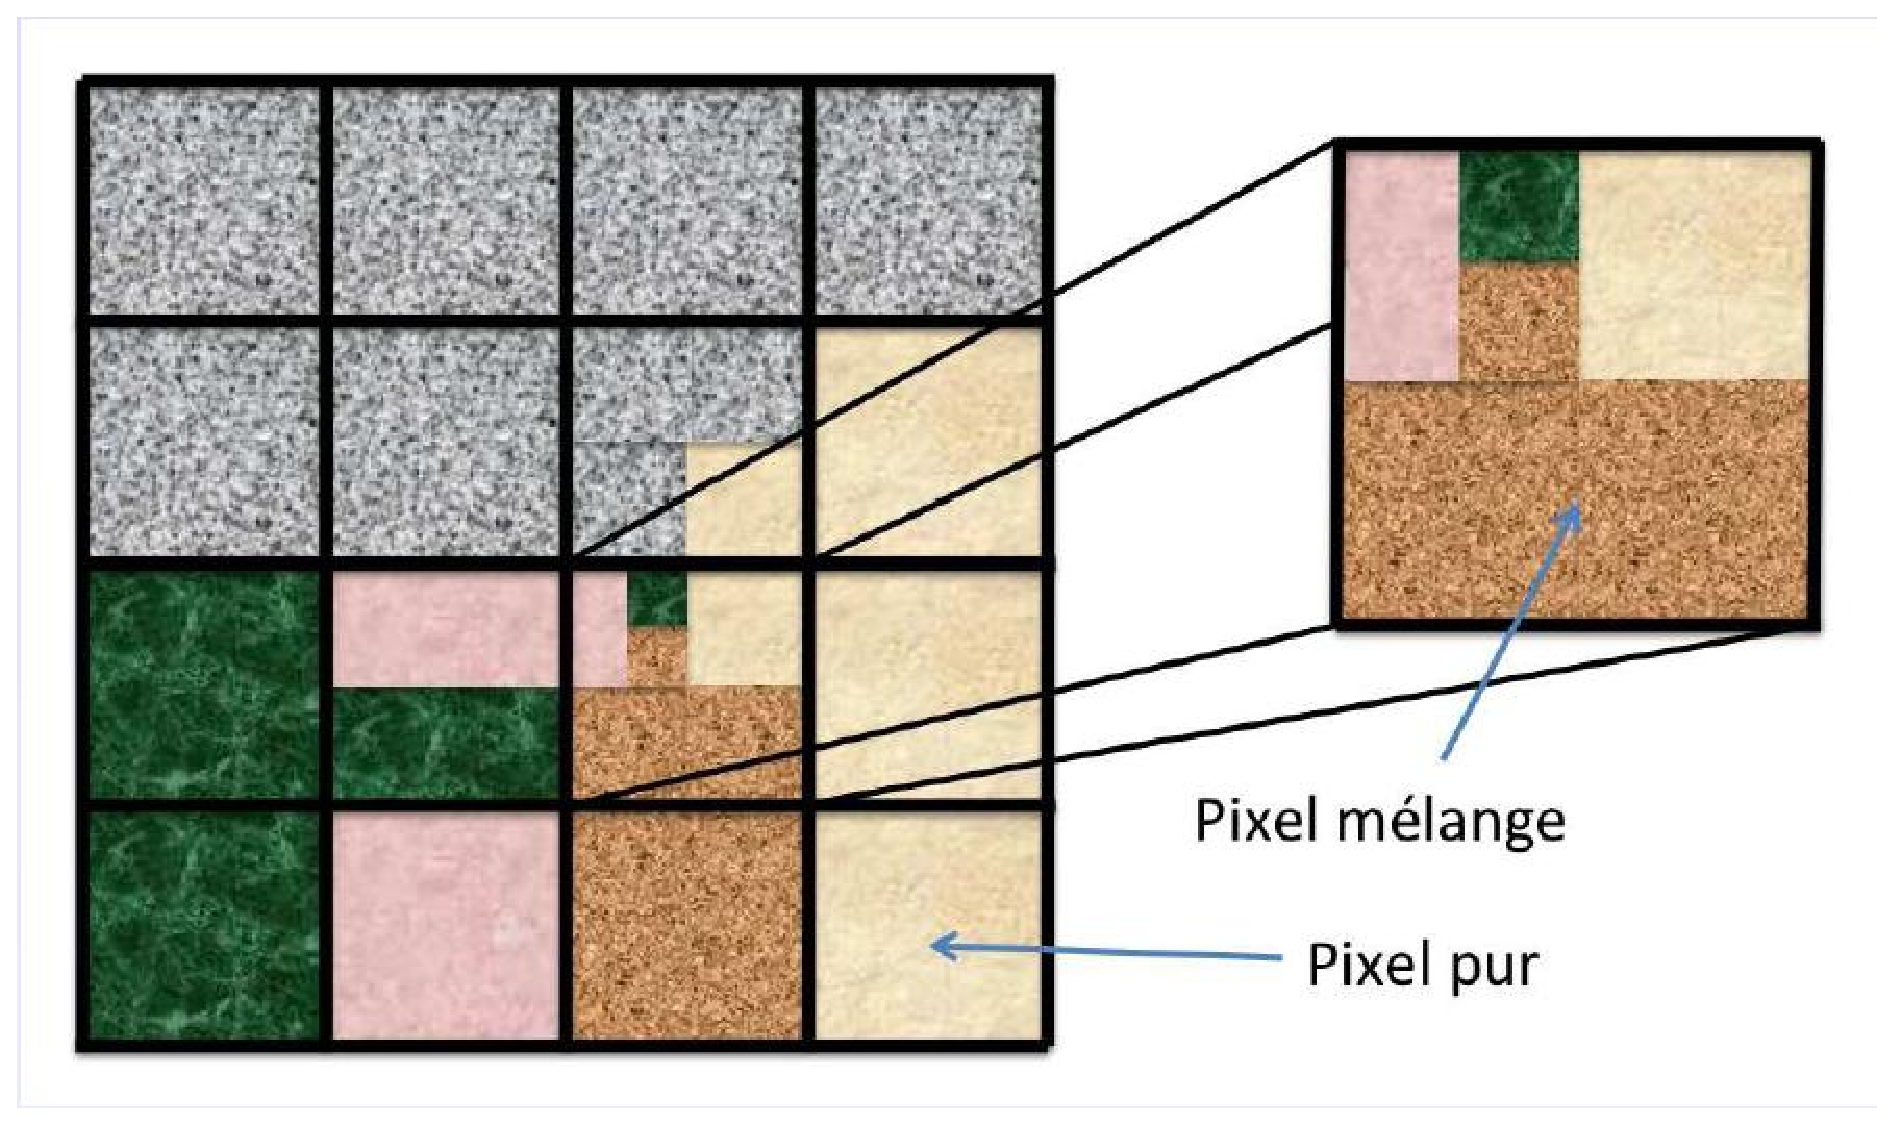
\includegraphics[width=0.7\textwidth]{Linear_Unmixing_HPX.eps}
  \itkcaption[Modele de melange linear]{ Schéma d'une zone vérifiant le modèle MML.}
  \label{fig:linear_unmixing}
\end{figure}

Nous notons \ref{fig:linear_unmixing}  la
présence de pixels-purs et de pixels-mélanges. Le MML admet que le
spectre de réflectance associé à chaque pixel est une combinaison
linéaire des spectres de matériaux purs composant la zone de
recouvrement, communément appelés ``endmembers''. Cela peut être
illustré \ref{fig:decomp_mml} :

\begin{figure}[h]
  \centering
  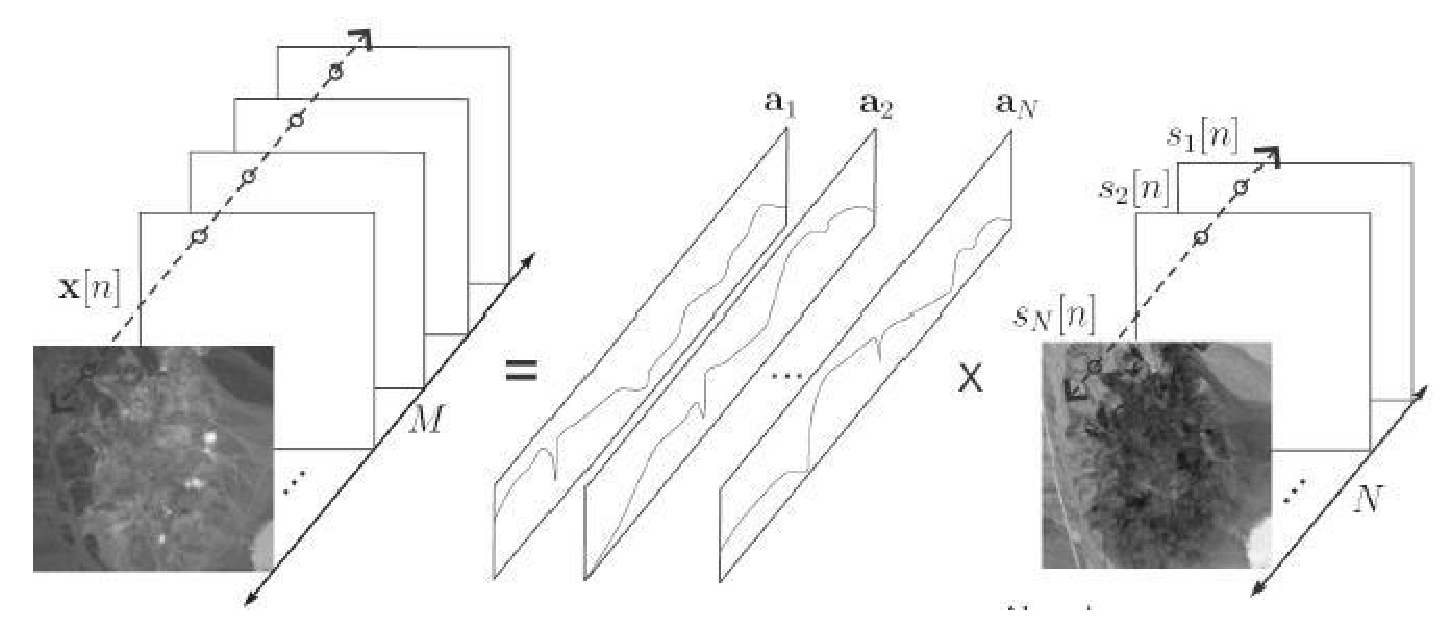
\includegraphics[width=0.7\textwidth]{Decomposition_MML_HPX.eps}
  \itkcaption[Decomposition Modele de melange linear]{Décomposition d'un cube hyperspectral selon le MML.}
  \label{fig:decomp_mml}
\end{figure}

Le ``terme'' de gauche représente les différentes bandes spectrales du
cube de données. Le ``terme'' de droite représente un ``produit''
entre les spectres de réflectance des endmembers et leurs cartes
d'abondances respectives. La carte d'abondance d'un endmembers est une
image en niveaux de gris compris entre $0$ et $1$. Le pixel i de la carte
d'abondance du endmember j a pour valeur $s_{ji}$. Cette valeur est
l'abondance du endmember j dans le pixel i. Sous certaines conditions
[Huck2009], cette valeur peut être interprétée comme le ratio
surfacique du matériau dans la zone de recouvrement (\ref{fig:linear_unmixing}).  En
pratique, on peut raisonnablement s'attendre: 

\begin{enumerate}
\item{à ce qu'un nombre
limité de matériaux purs composent la scène.}
\item{à ce que la scène
contienne des pixels purs si la résolution spatiale est suffisante, et
n'en contienne pas forcément sinon.}
\end{enumerate}
 
De nombreuses techniques d'analyse d'images hyperspectrales reposent
sur une approche géométrique ou chaque pixel spectral est vu comme un
vecteur de dimension L (nombre de bandes spectrales). Les
bandes spectrales peuvent alors être écrites sous forme vectorisée.

%% Figure 5: "Vectorisation" du cube hyperspectral. Les pixels spectraux
%% sont rangés dans les colonnes de la matrice R et, de manière
%% équivalente, les bandes spectrales sont rangées dans les lignes de R.

Par déduction de \ref{fig:decomp_mml} et de la Figure5, le MML consiste à décomposer R
de la manière suivante : $R= A.S + N = X + N$

Soit J le nombre de endmembers et I le nombre de pixels spectaux: 
\begin{enumerate}
\item{Les J colonnes de la matrice A contiennent les spectres de endmembers.}
\item{Les J lignes de la matrice S contiennent les cartes d'abondances
vectorisées;nous appelons vecteurs d'abondances les colonnes de la
matrice S.}
\item{La matrice N, de dimensions $LxI$, est une matrice de bruit
additif.}
\end{enumerate}

   

Le problème du démixage consiste à estimer les matrices A et S à
partir de R ou éventuellement de Xchapeau, une estimation de la matrice signal
débruité.

Remarque: Plusieurs contraintes physiques peuvent être prises en
compte pour permettre la résolution de ce problème: 
C1: positivité
des spectres de réflectance (matrice A non-négative); 
C2: positivité
des abondances (matrice S non-négative); 
C3: additivité des
abondances (la somme des coefficients de chaque colonne de la matrice
S vaut 1); 
L'indépendance algébrique entre les ``vecteurs spectraux''
associés au endmembers et la linéarité des mélanges de spectres, d'ou
découle la propriété du simplexe décrite au paragraphe suivant.
Simplexe circonscrit aux données Les algorithmes récents de démixage
s'appuient sur la ``propriété du simplexe''. Dans un espace vectoriel
de dimension $J-1$, on peut associer à J vecteurs algébriquement
indépendants J points définissant les sommets d'un J-simplexe, comme
l'illustre la Figure 6.

Figure 6: Illustration d'un 2-simplexe, d'un 3-simplexe et d'un
4-simplexe.  Un cube hyperspectral de L bandes, basé sur J endmembers,
peut être confiné dans un sous-espace-affine de dimension $J-1$.  Un
sous espace pertinent, au sens du rapport signal-a-bruit, est
généralement obtenu par Analyse en Composantes Principales (ACP). En
pratique, les $J-1$ vecteurs propres associés au plus fortes valeurs
propres forment les colonnes d'une matrice de projection V de
dimension $(Lx(J-1))$. Les données réduites Z, de dimensions $((J-1)xI)$,
sont obtenues par l'opération:

ou chaque colonne de'est vue soustraire le spectre moyen,
généralement estimé au sens du maximum de vraisemblance. Dans le
sous-espace porteur des vecteurs-colonnes de Z, les spectres de
endmembers sont donc associés au sommet d'un simplexe. Si le bruit est
négligeable, ce simplexe circonscrit les données réduites.

Remarque: Cette propriété met en évidence le fait que les endmembers
recherchés sont les sommets d'un simplexe qui circonscrit les
données. Cependant, une infinité de simplexes différents peuvent
circonscrire un même jeu de données. En fait, le problème du démixage
n'a généralement pas de solution unique. Cette dégénérescence peut
aussi être mise en évidence par le formalisme de la factorisation en
matrices non-négatives (voir Huck2010a), qui sera abordé un peu plus
loin. Il convient donc de choisir la solution physiquement la plus
pertinente. Toutes les techniques de démixage basées sur cette
propriété du simplexe admettent que la solution la plus pertinente est
définie par le simplexe admissible de volume minimal, ou la notion de
volume est généralisée à toutes les dimensions finies (éventuellement
différentes de 3).  Sélection d'algorithmes et état de l'art Les
algorithmes de démixage linéaire les plus récents exploitent
généralement la propriété du simplexe. Il est possible de les classer
en plusieurs familles: 
Famille 1 Une première famille d'algorithmes
de démixage est basée sur la recherche des endmembers ``parmi'' les
données. Cela signifie qu'un pixel pur au minimum doit etre associé à
chaque endmembers. Si cette hypothèse n'est pas vérifiée, cela
produira une erreur d'estimation sur les spectres de
endmembers. L'avantage historique de ces algorithmes est leur faible
complexité algorithmique. Les trois plus connus sont PPI (Pixel Purity
Index), NFINDER et VCA (Vertex Component Analysis)
[Nascimento2005]. Outre son succès reconnu par la communauté et sa
complexité algorithmique très compétitive, l'estimation des spectres
de endmembers est non biaisée en l'absence de bruit (et lorsque il y a
des pixels purs). Nous avons donc retenu cet algorithme pour l'étude.
VCA [Nascimento2005] 
Note: L'algorithme VCA est systématiquement
utilisé pour initialiser les différents algorithmes étudiés (sauf
MVES, basé sur une autre initialisation).

Eléments importants sur le fonctionnement de VCA: L'algorithme VCA
est basé sur des projections itératives des données orthogonales au
sous-espace porté par les endmembers déjà estimés; Biaisé lorsque le
degré de pureté est inférieur à 1; Famille 2 Une deuxième famille est
composée d'algorithmes recherchant le simplexe de volume minimal
circonscrivant les données. La phase d'initialisation consiste à
déterminer un simplexe initial quelconque circonscrivant les
données. Puis, un schéma d'optimisation numérique permet de minimiser
une fonctionnelle, fonction croissante du volume généralisé, lui-même
dépendant des endmembers estimés à l'itération
courante. L'optimisation est contrainte par le fait que les données
doivent restées inscrites dans le simplexe et éventuellement par les
contraintes C1, C2 et C3.

Les algorithmes considérés sont: MVSA (Minimum Volume Simplexe
Analysis) [Li2008]; MVES (Minimum Volume Encosing Simplex)
[Chan2009]; SISAL (Simplex Identification via Split Augmented
Lagrangian) [Dias2009]. 

Les différences principales entre les algorithmes considérés
concernent: 
Le schéma d'optimisation numérique; 
La manière dont les
contraintes sont prise en compte; 
Ces points impactent la complexité
algorithmique et la précision d'estimation.  MVSA aLi2008] Eléments
  importants sur le fonctionnement de MVSA: Initialisation par VCA;
  Tous les pixels spectraux inclus dans le simplexe estimé
  (approximativement) par VCA n'impactant pas la contrainte
  d'inscription des données dans le simplexe recherché, ils sont
  simplement supprimés des données utilisées dans la phase de
  minimisation du simplexe afin de réduire la complexité
  algorithmique.  La technique d'optimisation très évoluée est de type
  programmation quadratique séquentielle (Sequencial Quadratic
  Programming - SQP) et plus précisément à la catégorie
  ``quasi-Newton'' sous contrainte.  MVES [Chan2009] Eléments
  importants sur le fonctionnement de MVES: Initialisation par une
  méthode itérative (Programmation Linéaire LP pour Linear
  Programming) non-triviale et différente de VCA; Résolution du
  problème par LP.

  SISAL [Dias2009]
Eléments importants sur le fonctionnement de SISAL: Initialisation
par VCA; 
Sélection des pixels spectraux analogue à MVSA pour réduire
la complexité algorithmique; 
Technique d'optimisation très évoluée
cumulant plusieurs particularités: 
Décomposition du problème
non-convexe en série de problèmes convexes; 
Développement d'une
méthode spécifique de séparation de variables permettant de considérer
un lagrangien augmenté avec de bonnes propriétés de calcul.  
Famille 3
Il s'agit d'algorithmes de Factorisation en matrices non-négatives
(NMF pour Non-negative Matrix Factorization). L'objectif de cette
branche des mathématiques appliquées est de factoriser une matrice
non-négative, X dans notre cas, en produit de matrices
non-négatives:AS par minimisation d'une distance entre X et AS et
avec une régularisation adaptée, afin de lever la dégénérescence de
manière adaptée au problème physique associé au démixage.  MDMD-NMF
[Huck2010b] Eléments importants sur le fonctionnement de MDMD-NMF:
Initialisation par VCA; 
Minimisation de la norme de la norme de
Frobenius avec une régularisation spectrale et une régularisation
``spatiale'' (sur la matrice d'abondances).  
Minimum spectral
Dispersion: la régularisation spectrale encourage la variance des
coefficients d'un spectre de endmembers à être faible.  Maximum
spatial Dispersion: la régularisation spatiale encourage les vecteurs
d'abondances à occuper toute la partie admissible (plus d'information
dans [Huck2009]). Cette action présente une certaine analogie à la
contrainte de volume minimum.

Remarques complémentaires importantes Les algorithmes des familles 1
et 2 estiment les spectres de endmembers ``seulement''. L'estimation
des cartes d'abondances a lieu a posteriori et requiert l'application
d'un algorithme de type Fully Constrained Least Square (FCLS)
[Heinz2001]. MVES inclut un algorithme spécifique d'estimation des
abondances, que nous avons utilisé dans nos simulations (pour MVES
seulement).  Le démixage est un problème généralement non convexe, ce
qui explique l'importance de l'initialisation des algorithmes.
Récapitulatif de la prise en compte des différentes contraintes
physiques:

VCA MVSA MVES SISAL MDMD C1 $(A>0)$ muette Muette Muette Muette Dure C2
$(S>0)$ muette Dure Dure Souple Dure C3 (additivité) Muette (via FCLS)
Dure Dure Dure Souple simplexe Endmembers parmi les données
Circonscrit aux données Circonscrit aux données Circonscrit aux
données Indirecte par la régularisation ``spatiale'' Tableau 1:
Comment les différents algorithmes exploitent les c
%% \section{Dimensionality reduction}

%% \section{Anomaly detection}
%% Une anomalie dans une scène est, par définition, un élément qu'on ne
%% s'attend pas à y trouver. L'élément anormal est donc de nature
%% différente de son environnement et sa présence est minoritaire dans la
%% scène. Typiquement, un véhicule dans en milieu naturel, un rocher dans
%% champ, une cabane en bois dans une forêt suffisamment clairsemée sont
%% autant d'anomalies que l'on peut souhaiter détecter à l'aide
%% d'imagerie hyperspectrale. Cela suppose que la réponse spectrale de
%% l'anomalie puisse être discriminée de la réponse spectrale du
%% « fouilli-du-fond » (background clutter). Cela suppose également que
%% les pixels associés aux anomalies, les pixels anormaux, sont
%% suffisamment rares et/ou ponctuels pour pouvoir être considérés comme
%% tels. Ces propriétés peuvent être vues comme des hypothèses spectrales
%% et spatiales sur lesquelles s'appuient les techniques de détection
%% d'anomalies dans les images hyperspectrales.

%% Nous rappelons que la littérature relative à l'imagerie hyperspectrale
%% distingue généralement la détection de cibles et la détection
%% d'anomalies.  On parle de détection de cibles lorsque la réponse
%% spectrale de l'élément recherché est utilisée en entrée de
%% l'algorithme de détection. Il s'agit d'information a priori qui
%% permet, en théorie, de construire des algorithmes à très fort pouvoir
%% de détection, tels que l'Adaptive Matched Filter (AMF) ou l'Adaptive
%% Cosine/Coherence Estimator (ACE),pour n'en citer que deux. Néanmoins,
%% la connaissance suffisamment fine du spectre recherché est une
%% information difficile à détenir en pratique, ce qui conduit bien
%% souvent à l'utilisation d'algorithmes de détection d'anomalies.  On
%% parle de détection d'anomalies lorsque le spectre de l'élément anormal
%% n'est pas requis par l'algorithme de détection. Pour cette raison, on
%% associe souvent le terme de « détection non supervisée ». Néanmoins,
%% les algorithmes dépendent généralement de « paramètres de
%%   structure ». Par exemple, dans le cas de la détection dans une
%% fenêtre glissante, le juste choix des dimensions repose sur une
%% connaissance a priori de la taille des anomalies recherchées. Cette
%% partie de l'étude se concentre sur la comparaison d'algorithmes de
%% détection d'anomalies.

%% Dans la Figure 26, nous introduisons d'ores et déjà quelques notions
%% qui seront utiles par la suite. Les algorithmes de détection
%% d'anomalies ont comme entrée une image et estiment une carte de
%% détection faisant office d'outil d'aide à la prise de décision. Un
%% seuillage adapté permet d'obtenir un masque de détection estimé, que
%% l'on espère le plus ressemblant possible au masque de vérité terrain,
%% inconnu en pratique. Ce masque estimé a la vocation d'un outil de
%% prises automatiques de décisions.

%% Figure 26: Notions sur la détection: masque de vérité terrain, carte
%% de détection, masque de détection.

%% Deux approches dominent l'état de l'art sur la détection d'anomalies
%% dans les images hyperspectrales. Il s'agit des méthodes par Poursuite
%% de Projection (PP) et les méthodes basées sur une modélisation
%% probabiliste de la classe fond et éventuellement de la classe cible
%% avec test d'hypothèses statistiques.  La PP consiste à projeter
%% linéairement les pixels spectraux sur des vecteurs wi qui optimise un
%% critère sensible à la présence d'anomalies (ex: kurtosis). On obtient
%% une série de cartes de projections où les anomalies contrastent très
%% fortement avec le fond. Mais l'estimation automatique d'une carte de
%% détection présente des difficultés majeures, notamment: Combien de
%% projecteurs doit-on estimer ?  Quel(s) projecteur(s) choisir?  Comment
%% gérer un fond inhomogène ?  Les performances de détection varient avec
%% les dimensions spatiales de l'image (nombre d'échantillons); Ces
%% algorithmes ont généralement une structure peu parallélisable ; Ces
%% algorithmes ne sont généralement pas « à taux de fausse alarme
%%   constant ».

%% Ces difficultés nous ont conduit à considérer, dans le cadre de cette
%% R&T, exclusivement des algorithmes de la deuxième catégorie évoquée,
%% basés sur les notions de modèles probabilistes, test d'hypothèses
%% statistiques et fenêtre glissante. Les algorithmes retenus sont
%% présentés dans la partie suivante.  Algorithmes sélectionnés Les
%% algorithmes sélectionnés sont RX (présenté en première version dans
%% [Reed1990] et GMRF [Schweizer2001] et leurs spécificités respectives
%% seront présentées plus loin. Ils sont basés sur les notions de modèles
%% probabilistes, test d'hypothèses statistiques et fenêtre glissante.
%% Ce type d'approche consiste à répondre à la question : « Le pixel (ou
%%   ensemble de pixels voisins) testé ressemble-t-il au pixels du
%%   fond? » par une démarche de test statistique. De manière plus
%% exhaustive, cette démarche nécessite : Un modèle pour la classe
%% « fond »; Le choix d'un test statistique; Éventuellement, un modèle
%% pour la classe « anomalie »; Des estimateurs pour les différents
%% paramètres inconnus a priori; Des hypothèses d'homogénéité permettant
%% un compromis satisfaisant entre: Le nombre d'échantillons en regard du
%% nombre de paramètres à estimer; L'homogénéité, notamment du fond; La
%% complexité algorithmique (quoique les algorithmes considérés sont
%% hautement parallélisables);

%% Le principe de fonctionnement de RX et GLRT peut être résumé par les
%% Figure 27 et Figure 28.

%% Figure 27: Schéma bloc des algorithmes considérés.  Une première étape
%% facultative (spontanément considérée dans le cadre de cette R&T)
%% consiste à réduire la dimension spectrale des données tout en
%% conservant l'information liée aux anomalies. Puis, les pixels
%% spectraux sont testés à tour de rôle (tâche parallélisable). Le pixel
%% testé se voit attribuer une fenêtre glissante (voir Figure 28). Cette
%% fenêtre comprend deux sous fenêtres, centrées sur le pixel testé, de
%% dimensions respectives L et LL, avec L < LL.  Les pixels appartenant à
%% la couronne ainsi formée appartiennent à la classe « fond local ». Les
%% paramètres statistiques du fond, requis par les tests statistiques,
%% sont estimés à partir de ces pixels spectraux. L'une des difficultés
%% consiste à trouver un compromis sur l'épaisseur de la couronne (et
%% donc le nombre d'échantillons statistiques) sachant que : Si la
%% couronne est trop épaisse, le fond local n'est plus suffisamment
%% homogène ; Si le nombre d'échantillons est trop faible, la précision
%% de l'estimation statistique des paramètres du modèle du fond est trop
%% faible.  Les pixels de la partie centrale de la fenêtre glissante
%% appartiennent à la classe « inconnue ». Si le pixel testé (pixel
%% central) est un pixel anormal, il est possible que ses voisins soient
%% aussi des pixels anormaux, d'où l'intérêt de ne pas choisir une valeur
%% de L trop faible si l'on sait que les anomalies recherchées peuvent
%% être réparties sur plusieurs pixels.  Une fois l'ensemble des
%% paramètres estimés, un test statistique est effectué et affecte une
%% valeur Λ(i) au pixel testé i. Une carte de détection est ainsi
%% constituée.

%% Figure 28: Principe de la fenêtre glissante et définitions des
%% paramètres L et LL de la fenêtre glissante.  Les algorithmes RX et
%% GMRF, considérés dans présentés dans les sections suivantes.

%% \subsection{Local RX}
